\PassOptionsToPackage{quiet}{fontspec}
\documentclass[12pt,a4paper,UTF8]{article}
\usepackage{thesis} % 格式控制
\usepackage{indentfirst}
\usepackage{enumitem}
\usepackage{float}
\usepackage{array}
\usepackage{longtable}
\usepackage{xltabular}
\usepackage{etoolbox}


\setlength{\parindent}{2em} % 控制首行缩进  
\addtolength{\parskip}{3pt} % 控制段落距离  
\onehalfspacing % 1.5倍行距  
\graphicspath{{./figures/}} % 指定图片所在文件夹  


\classname{软件工程}  % 设置课程名称
\makepagestyle{}{\printclassname ~:项目开发计划书}




\begin{document}
\maketitlepage{项目开发计划书}{动物领养系统}{尹建伟}{计算机科学与技术学院}{}{}{} 

\maketoc    %目录页

\section{引言} 

\subsection{编写目的}

本文档是浙江大学计算机学院软件工程课程的项目设计——动物领养系统的开发计划书,旨在为动物领养系统的开发工作提供全面、清晰的指导。其主要目的包括:明确项目的内容与产出、规划开发流程与人员安排、风险评估与应对策略制定,以及支持条件的分析等等

\subsection{项目背景}

\subsubsection{社会背景}
随着社会的发展和人们生活水平的提高,越来越多的人开始关注动物保护和领养问题。流浪动物的数量不断增加,不仅给城市的环境卫生和公共安全带来挑战,也引发了社会各界对动物福利的广泛关注。传统的动物救助方式主要依赖于志愿者的线下活动和动物收容所的有限资源,但这些方式存在诸多局限性,如信息传播范围有限、领养流程繁琐、缺乏有效的跟踪和反馈机制等。因此,开发一个高效、便捷的动物领养系统,对于改善流浪动物的生存状况、提升动物保护工作的效率和效果具有重要意义。

\subsubsection{行业现状}
目前,虽然市场上已经存在一些动物救助和领养相关的平台,但这些平台大多功能单一、信息更新不及时、用户体验不佳,许多动物收容所和志愿者组织仍然依赖于社交媒体或线下宣传来寻找潜在的领养者。因此,开发一个功能全面、操作便捷、服务完善的动物领养系统,能够填补市场空白,满足动物保护行业发展的需求。

\section{项目概述}

\subsection{工作内容}

\subsubsection{项目的规模}

\begin{enumerate}
  \item \textbf{系统功能范围} \\
  主要涵盖基础信息模块、动物领养申请模块、动物地图定位模块这三个功能模块,在需求分析书中有具体介绍
  \item \textbf{预期用户规模} 
  \begin{itemize}
    \item 动物救助组织和志愿者管理员:预计系统上线初期将有1家动物救助组织(浙江大学学生动物保护者协会)和100名志愿者注册使用该系统,随着项目的推广和影响力的扩大,预计一年内用户数量将增长至10家救助组织和1000名志愿者。
    \item 潜在领养者:在系统推广初期,预计每月将有30名潜在领养者访问系统并进行领养申请,随着系统的知名度提升和用户口碑传播,预计一年后月均领养申请量将达到300份以上。
    \item 服务提供商:计划在系统上线初期与3家动物医院、宠物店等服务提供商建立合作关系,随着系统用户规模的扩大,预计一年内合作的服务提供商数量将增加至10家以上。
  \end{itemize}
  \item \textbf{数据量预估} 
  \begin{itemize}
    \item 动物信息数据:系统上线初期预计录入200余只待领养动物的信息,随着项目的推进和更多救助组织的加入,预计一年内动物信息数据量将达到2000条以上。
    \item 用户数据:包括救助组织、志愿者、领养者等各类用户的数据,预计系统上线一年后用户数据总量将达到1000条以上。
    \item 领养申请数据:根据预期的领养申请量,系统上线初期每月将产生约30条领养申请数据,一年后月均领养申请数据量预计将达到300条以上。
  \end{itemize}
  \item \textbf{开发工作量} \\
  迭代周期为每4周一次,后端设计2人/周期,前端设计2人/周期,前后端合并测试1人/周期,文档跟进及测试3人/周期。估算共需4个迭代周期,共16周。
\end{enumerate}

\subsubsection{项目的软件生命周期及模型}

我们选取敏捷模型为该项目的软件生命周期,主要是基于以下考虑:
\begin{itemize}
  \item 需求的不确定性:动物领养系统的用户需求可能在开发过程中发生变化。敏捷模型能够快速响应需求变更,确保系统开发与用户需求保持一致。
  \item 快速交付与迭代:敏捷开发强调快速交付可用的软件版本,通过持续的迭代和反馈,逐步完善系统功能。这有助于及时发现和解决问题,提高系统的质量和用户体验。
  \item 团队协作与沟通:敏捷开发注重团队成员之间的紧密协作和高效沟通,能够充分发挥团队成员的创造力和积极性。
\end{itemize}

它主要分为这几个阶段:需求——计划——开发——测试——回顾,具体的软件生命周期及模型如下图所示:

\begin{figure}[!htbp]
  \centering
  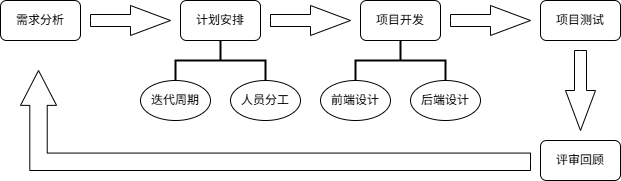
\includegraphics[width=0.9\textwidth]{figures/process_model.png}
\end{figure}

\subsubsection{项目的软件功能}

为了满足系统的要求,动物领养系统的功能模型如下图所示:
\begin{figure}[!htbp]
  \centering
  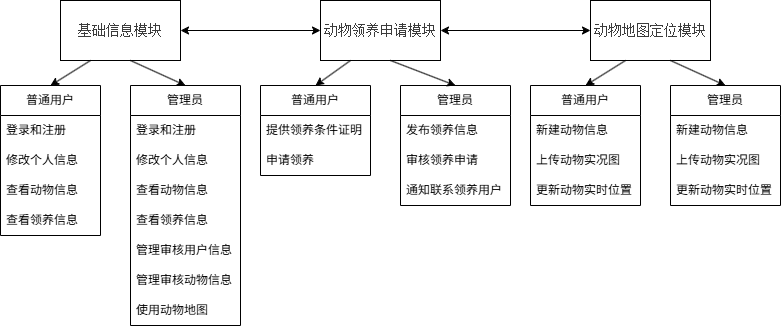
\includegraphics[width=0.9\textwidth]{figures/function_model.png}
\end{figure}

\begin{enumerate}
  \item \textbf{基础信息模块} \\
  面向用户:
  \begin{itemize}
    \item 注册与登录:用户在注册界面输入手机号和密码,验证通过后完成注册。已注册用户在登录界面正确输入手机号/账号及密码后,即可进入用户主页;若账号不存在或手机号未注册,提示注册;若密码错误,提示重新输入或提供找回密码选项
    \item 查看/修改个人信息:用户在进入个人主页后,可进行操作包括查看个人信息(昵称、地址、养宠经验等)、查看领养申请状态、修改用户名、密码、手机号、地址等信息
    \item 查看动物信息:用户可以在动物列表或搜索结果中查看待领养动物的详细信息,包括照片、种类、品种、健康状况、性格描述、当前位置等
    \item 提交/更新动物信息:用户发现流浪动物后,可以提交新的动物信息(包括照片、发现地点、基本描述),等待管理员审核。对于已存在的动物,用户可以更新其位置信息
    \item 使用动物识图:用户可以通过拍照或上传本地图片的方式,尝试识别遇到的动物,系统返回可能的种类、品种以及系统内相似的动物信息
  \end{itemize}
  面向管理员:
  \begin{itemize}
    \item 登录:管理员在登录界面正确输入管理员账号及密码后,即可进入管理后台;若账号错误,提示重新输入;若密码错误,提示重新输入或忘记/修改密码
    \item 查看/修改个人信息:管理员在进入管理后台后,可进行操作包括查看待办事项(如待审核信息)、修改管理员账户信息
    \item 审核/管理用户信息:管理员可以查看普通用户列表,审核用户提交的个人信息修改请求,管理用户账户状态
    \item 发布/审核/管理动物信息:管理员可以发布新的待领养动物信息,审核用户提交的动物信息,编辑已有的动物信息,更新动物的领养状态
    \item 查看/更新动物地图:管理员可以查看动物地图,了解所有已记录动物的分布情况,并可以更新或修正动物的位置信息
  \end{itemize}
  \item \textbf{动物领养申请模块} \\
  面向用户:
  \begin{itemize}
    \item 提交/查看领养申请:用户对心仪的动物可以提交领养申请,填写必要的申请信息或问卷。用户可以在个人中心查看自己提交的所有领养申请及其当前的审核状态(待审核、已批准、已拒绝)
    \item 查看领养指南:用户可以浏览、搜索管理员发布的领养指南、教程和相关知识
  \end{itemize}
  面向管理员:
  \begin{itemize}
    \item 审核/管理领养申请:管理员可以查看所有待审核的领养申请,查看申请人信息和申请材料,进行批准或拒绝操作,并填写审核意见
    \item 发布/管理领养指南:管理员可以发布、编辑领养指南和相关知识文章
  \end{itemize}
  \item \textbf{动物地图定位模块} \\
  面向用户:
  \begin{itemize}
    \item 更新动物地图:用户在遇到流浪动物时,可以先通过动物识图进行识别,在系统中找到匹配对象,然后更新该动物的位置信息;如果匹配失败,可以新建动物信息,并上传实况图方便后续识别
  \end{itemize}
  面向管理员:
  \begin{itemize}
    \item 查看/更新动物地图:管理员可以查看动物地图,了解所有已记录动物的分布情况,并可以更新或修正动物的位置信息
  \end{itemize}
\end{enumerate}

\subsubsection{项目的软件性能}

系统的性能可以从以下方面来衡量(作为后续测试的指标):
\begin{enumerate}
  \item \textbf{界面设计}:系统的UI应简洁直观,布局合理,清晰地呈现信息,突出重点内容。操作方便,用户容易上手
  \item \textbf{响应速度}:系统具有良好的反应速度,给用户良好的使用体验。我们要求在良好的网络情况下,系统应具有以下时间特性要求:
  \begin{itemize}
      \item 单个用户在线时:
      \begin{itemize}
          \item web 页面加载及用户操作响应时间小于 1 秒
          \item 动物信息搜索、地图加载操作响应用户动作时间小于 3 秒
          \item 图像识别响应时间(从上传到返回结果)小于 10 秒
      \end{itemize}
      \item 100 个用户同时在线时:
      \begin{itemize}
          \item web 页面加载及用户操作响应时间小于 2 秒
          \item 动物信息搜索、地图加载操作响应用户动作时间小于 5 秒
      \end{itemize}
  \end{itemize}
  \item \textbf{访问容量}:该系统至少在同一时间内支持 500 个用户并发访问
  \item \textbf{服务器配置最低要求}:CPU Dual Core 2.5GHz,内存 8G,硬盘 SSD
  \item \textbf{数据处理能力}:至少支持 10000 条用户数据,至少支持 20000 条动物数据,至少支持其余类型数据(申请、位置、指南等)各 50000 条
  \item \textbf{可用性}:该系统应实现多 web 浏览器支持:在大多数流行的 web 浏览器中正确显示和执行,包括 Firefox、Chrome、Edge 等
\end{enumerate}

\subsection{条件和限制}

\subsubsection{条件}

\begin{enumerate}
  \item \textbf{技术条件} 
  \begin{itemize}
    \item 开发环境:项目开发团队需要具备稳定的开发环境,包括但不限于开发工具、测试工具、版本控制系统等。所有开发人员需熟练掌握项目所采用的技术栈,如前端技术(React、Vue等)、后端技术(Spring Boot、Node.js等)和数据库技术(MySQL、PostgreSQL等)。
    \item 网络安全:系统涉及用户数据和动物信息,必须确保网络安全,防止数据泄露和恶意攻击。开发团队需遵循网络安全最佳实践,如采用SSL/TLS加密、防火墙设置、入侵检测系统等。
  \end{itemize}
  \item \textbf{人员条件}
  \begin{itemize}
    \item 人员稳定性:项目开发周期预计为16周,团队成员需保持相对稳定,避免因人员变动导致项目进度延误。
    \item 讨论与学习:团队成员需具备快速学习和适应新技术的能力,定期召开会议进行讨论,汇报进度,督促团队。
  \end{itemize}
\end{enumerate}

\subsubsection{限制}

\begin{enumerate}
  \item \textbf{时间限制} \\
  项目开发周期为16周,项目团队需在每个里程碑节点前完成相应的工作内容,并进行阶段性的评审和验收。关键里程碑包括需求分析完成、系统设计完成、开发阶段完成、测试阶段完成等。
  \item \textbf{法律和政策限制}
  \begin{itemize}
    \item 数据保护法规:系统涉及用户个人信息和动物信息,需严格遵守相关数据保护法规,如《中华人民共和国网络安全法》《中华人民共和国数据安全法》等,确保用户数据的合法收集、存储、使用和传输。
    \item 动物保护政策:项目需符合国家和地方的动物保护政策,确保系统功能和运营符合法律法规要求,不涉及任何违法或不当的动物交易行为。
    \item 知识产权保护:项目开发过程中需尊重知识产权,确保所使用的软件、技术、数据等均为合法授权或开源许可。同时,项目团队需保护自身开发的软件和知识产权,避免侵权行为。
  \end{itemize}
  \item \textbf{市场和用户限制}
  \begin{itemize}
    \item 用户需求变化:项目开发过程中需密切关注用户需求的变化,及时调整系统功能和设计。
    \item 市场竞争:市场上已存在一些动物领养相关的平台,项目需在功能、用户体验、服务质量等方面具有竞争优势,才能吸引用户使用。
  \end{itemize}
\end{enumerate}

\subsection{产品}

\subsubsection{程序}
\verb|ChaMaoMao| 动物领养系统

\subsubsection{文档}
\begin{enumerate}
  \item \textbf{会议记录} \\
  项目开发过程中每两周进行一次会议讨论,进行会议记录。如有临时会议也需要进行会议记录。格式为《yyyy-mm-dd.md》。
  \item \textbf{迭代记录} \\
  项目开发过程中每四周进行一次迭代,迭代记录提供本次迭代已完成的任务及布置下次迭代需要完成的需求。格式为《第x轮迭代.md》
  \item \textbf{过程文档} \\
  为课程要求,主要包括《需求分析书》、《项目开发计划书》等等
\end{enumerate}

\subsubsection{运行环境}

\begin{enumerate}
  \item \textbf{服务端}
  
  \verb|node.js| 版本:\verb|20.15.1|

  数据库: \verb|mysql 8.0.41|

  依赖要求: 

  \vspace{0.25cm} % 添加垂直间距

  \begin{lstlisting}
  <dependencies>

    <dependency>
      <groupId>mysql</groupId>
      <artifactId>mysql-connector-java</artifactId>
      <version>8.0.31</version>
    </dependency>

    <dependency>
      <groupId>org.opengauss</groupId>
      <artifactId>opengauss-jdbc</artifactId>
      <version>3.1.0</version>
      <scope>provided</scope>
    </dependency>

    <dependency>
      <groupId>com.microsoft.sqlserver</groupId>
      <artifactId>mssql-jdbc</artifactId>
      <version>12.2.0.jre8</version>
    </dependency>

    <dependency>
      <groupId>junit</groupId>
      <artifactId>junit</artifactId>
      <version>4.13.2</version>
      <scope>test</scope>
    </dependency>

    <dependency>
      <groupId>org.projectlombok</groupId>
      <artifactId>lombok</artifactId>
      <version>1.18.24</version>
      <scope>provided</scope>
    </dependency>

    <dependency>
      <groupId>com.google.code.gson</groupId>
      <artifactId>gson</artifactId>
      <version>2.9.1</version>
    </dependency>

    <dependency>
      <groupId>org.apache.commons</groupId>
      <artifactId>commons-lang3</artifactId>
      <version>3.7</version>
    </dependency>

  </dependencies>
  \end{lstlisting}
  \item \textbf{设备要求}
  
  浏览器要求:\verb|Chrome|、\verb|Edge|、\verb|Firefox| 等主流浏览器

  \verb|Windows|:\verb|11|

  \verb|MacOS|:\verb|13.0.1|

  \verb|Ubuntu|:\verb|22.04|
  \item \textbf{前端依赖}
  
  依赖要求:

  \vspace{0.25cm} % 添加垂直间距

  \begin{lstlisting}
    "dependencies": {
      "@element-plus/icons-vue": "^2.3.1",
      "axios": "^1.7.2",
      "element-plus": "2.6.0",
      "pinia": "^2.1.7",
      "vue": "^3.4.29",
      "vue-router": "^4.2.5",
      "vuex": "^4.1.0"
    },
    "devDependencies": {
      "@vitejs/plugin-vue": "^5.0.5",
      "vite": "^5.3.1"
    }
  \end{lstlisting}
  \item \textbf{客户端}
  
  \verb|Web| 应用,要求使用 \verb|Chrome|、\verb|Edge|、\verb|Firefox| 等主流浏览器访问
\end{enumerate}

\subsubsection{验收标准}

产品应达到立项时提出的2个目标,即:
\begin{enumerate}
  \item 完成需求分析书中所列出的各项功能;
  \item 提交课程要求所列的各项需要提交的文档;
\end{enumerate}

\section{实施计划}

\subsection{任务分解}

\begin{xltabular}{\linewidth}{|>{\centering\arraybackslash}p{2.2cm}|>{\centering\arraybackslash}p{2cm}|>{\raggedright\arraybackslash}p{6cm}|>{\centering\arraybackslash}p{1.5cm}|>{\centering\arraybackslash}p{2cm}|}
  \hline
  \textbf{阶段} & \textbf{任务编号} & \textbf{任务} & \textbf{负责人} & \textbf{截止日期} \\ \hline 
  \endfirsthead
  
  \hline
  \textbf{阶段} & \textbf{任务编号} & \textbf{任务} & \textbf{负责人} & \textbf{截止日期} \\ \hline  
  \endhead
  
  \hline
  \multicolumn{5}{r}{续下页} \\ 
  \endfoot

  \hline \endlastfoot

  第一次会议 & 会议1 & 
  \vspace{-0.5em}
  \begin{itemize}[topsep=0pt, partopsep=0pt, left=0pt, nosep]
    \item 确认项目内容为动物领养系统
    \item 进行初步的需求分析,大致敲定需要实现的功能
    \item 确认前端框架为vue,后端框架为springboot
    \item 进行初步的分工
  \end{itemize}
  & 金俊一 吴岱阳 & 3月24日 \\ \hline
  第一轮迭代 & 文案1-1 & 完成项目开发计划书 & 王宇飞 & 4月7日 \\ \hline
  第一轮迭代 & 文案1-2 & 完成需求分析书 & 王嘉成 & 4月7日 \\ \hline
  第一轮迭代 & 前端1-1 & 完成主要UI界面设计(包括主页、动物信息页面、动物地图界面等) & 吴岱阳 & 3月31日 \\ \hline
  第一轮迭代 & 后端1-1 & 实现基本API(包括动物信息类、用户信息类等等) & 季海川 陶卓 & 4月7日 \\ \hline
  第一轮迭代 & 测试1-1 & 设计测试路径 & 金俊一 & 4月7日 \\ \hline
  第二次会议 & 会议2 & 进度对齐,确认第二轮迭代目标 & 金俊一 吴岱阳 & 4月7日 \\ \hline
  第二轮迭代 & 文案2-1 & 完成展示PPT,准备需求评审 & 濮学易 & 4月28日 \\ \hline
  第二轮迭代 & 前端2-1 & 完成原型设计:使用工具(如Sketch、Figma、Axure等)创建系统的交互原型,展示页面布局、组件交互和用户操作流程 & 吴岱阳 鲁悦 & 4月21日 \\ \hline
  第二轮迭代 & 前端2-2 & 完成组件开发:开发通用组件(导航栏、按钮、信息输入框等),确保组件的复用性和可维护性 & 吴岱阳 鲁悦 & 4月28日 \\ \hline
  第二轮迭代 & 后端2-1 & 完成数据库设计,包括:
  \begin{itemize}[topsep=0pt, partopsep=0pt, left=0pt, nosep]
    \item 概念模型设计:根据需求分析,设计系统的概念模型(ER图),明确实体、关系和属性。
    \item 逻辑模型设计:将概念模型转化为逻辑模型,设计数据库表结构、字段类型、主键、外键等。
    \item 实现系统的业务逻辑,包括数据的增删改查、业务规则的校验、数据的关联查询等。
  \end{itemize}
  & 季海川 陶卓 & 4月21日 \\ \hline
  第二轮迭代 & 后端2-2 & 完成基础信息模块 & 季海川 陶卓 & 4月28日 \\ \hline
  第二轮迭代 & 测试2-1 & 等前后端联调完成后,测试登录逻辑 & 金俊一 & 4月28日 \\ \hline
  第二轮迭代 & 测试2-2 & 编写单元测试用例,对后端代码进行测试,确保代码的正确性和稳定性 & 金俊一 & 4月28日 \\ \hline
  第三次会议 & 会议3 & 进度对齐,确认第三轮迭代目标 & 金俊一 吴岱阳 & 4月28日 \\ \hline
  第三轮迭代 & 文案3-1 & 完成系统设计报告,准备系统设计评审 & 王宇飞 王嘉成 濮学易 & 5月12日 \\ \hline
  第三轮迭代 & 前端3-1 & 完成交互实现:实现页面的交互功能,如表单验证、动态加载数据、弹窗提示等,提升用户体验 & 吴岱阳 鲁悦 & 5月5日 \\ \hline
  第三轮迭代 & 前端3-2 & 完成API对接:与后端团队合作,根据后端提供的API文档,完成前端与后端的数据交互,确保数据的正确获取和提交 & 吴岱阳 鲁悦 & 5月12日 \\ \hline
  第三轮迭代 & 前端3-3 & 完成性能优化:优化前端代码,减少页面加载时间,提升系统性能。包括代码压缩、图片优化、懒加载等 & 吴岱阳 鲁悦 & 5月19日 \\ \hline
  第三轮迭代 & 后端3-1 & 完成动物领养申请模块 & 季海川 陶卓 & 5月5日 \\ \hline
  第三轮迭代 & 后端3-2 & 完成动物地图定位模块 & 季海川 陶卓 & 5月5日 \\ \hline
  第三轮迭代 & 后端3-3 & 完成API文档编写,包括接口地址、请求方法、参数说明、返回值等,方便前端团队对接 & 季海川 陶卓 & 5月12日 \\ \hline
  第三轮迭代 & 测试3-1 & 对前端开发的功能进行测试,确保页面布局、交互功能、数据加载等符合设计要求 & 金俊一 & 5月8日 \\ \hline
  第三轮迭代 & 测试3-2 & 进行兼容性测试,确保系统在主流浏览器(如Chrome、Firefox、Edge等)和不同操作系统上具有良好的兼容性 & 金俊一 & 5月15日 \\ \hline
  第四次会议 & 会议4 & 进度对齐,确认第四轮迭代目标 & 金俊一 吴岱阳 & 5月19日 \\ \hline
  第四轮迭代 & 文案4-1 & 完成测试报告和PPT,准备最终验收 & 王宇飞 王嘉成 濮学易 & 5月30日 \\ \hline
  第四轮迭代 & 前端4-1 & 根据测试结果进行相应改进 & 吴岱阳 鲁悦 & 6月2日 \\ \hline
  第四轮迭代 & 后端4-1 & 根据测试结果进行相应改进 & 季海川 陶卓 & 6月2日 \\ \hline
  第四轮迭代 & 测试4-1 & 编写测试脚本,模拟用户的完整操作流程,确保整个系统从前端到后端正常工作。同时考虑系统在各种情境下的性能,提出问题,交由前后端团队进行改进 & 金俊一 & 5月8日 \\ \hline
\end{xltabular}

\subsection{人员}
\begin{itemize}
  \item 王宇飞、王嘉成、濮学易——负责项目的文档撰写以及课程验收
  \item 吴岱阳、鲁悦——负责项目的前端设计
  \item 季海川、陶卓——负责项目的后端设计
  \item 金俊一——负责项目的测试工作,以及整个项目的协调与组织
\end{itemize}

\subsection{进度}

\begin{xltabular}{\linewidth}{|>{\centering\arraybackslash}p{4cm}|>{\centering\arraybackslash}p{4cm}|>{\centering\arraybackslash}p{4cm}|}
  \hline
  \textbf{阶段} & \textbf{起始时间} & \textbf{完成时间} \\ \hline 
  \endfirsthead
  
  \hline
  \textbf{阶段} & \textbf{起始时间} & \textbf{完成时间} \\ \hline  
  \endhead
  
  \hline
  \multicolumn{3}{r}{续下页} \\ 
  \endfoot

  \hline \endlastfoot

  立项、需求阶段 & 2025年3月17日 & 2025年3月31日 \\ \hline
  计划、概要设计阶段 & 2025年3月24日 & 2025年4月7日 \\ \hline
  编码阶段 & 2025年4月7日 & 2025年6月2日 \\ \hline
  测试阶段 & 2025年4月21日 & 2025年6月9日 \\ \hline
  验收阶段 & 2025年6月9日 & 2025年6月16日 \\ \hline
\end{xltabular}

\subsection{关键问题}

\subsubsection{风险分析及规避手段}
\begin{itemize}
  \item \textbf{人员风险}:本项目开发人员均为浙江大学本科学生,大家都面临着课业、科研、实习的压力,时间比较紧张。因此,在人员管理方面会比较困难,有时候会议也难以约定到统一的时间,可能出现无法及时完成规定任务的情况。这一风险的规避方法是:进行多轮迭代,碎片化项目开发任务,灵活分配工作,并且及时跟进工作进度。
  \item \textbf{技术风险}:开发人员是第一次开发此规模的软件,所以在技术和规范上都不是特别熟练,导致开发过程中可能遇到技术难题,如新技术的学习和应用、技术架构的优化等,容易产生技术风险。这一风险的规避方法是:明确小需求的实现方向,进行code review,使用eslint, husky等工具规范代码和commit信息。并且在项目开始前进行技术预研,评估技术可行性,确保团队具备解决技术难题的能力。
  \item \textbf{市场与用户风险}:
  \begin{itemize}
    \item 用户接受度低:部分用户可能更倾向于购买宠物而非领养,导致系统用户量不足。
    \item 信息不对称:用户上传的动物信息可能不准确或不全面,影响用户决策。
    \item 市场竞争激烈:市场上已有类似平台,我们开发的系统可能面临较大的竞争压力。
  \end{itemize}
  对应的规避手段为:
  \begin{itemize}
    \item 提升用户体验:优化系统界面和功能,提升用户满意度。并且建立反馈渠道,及时收集和处理用户意见,持续优化系统。
    \item 严格信息审核:建立严格的信息审核机制,确保救助机构和用户发布的信息真实可靠。
    \item 加强市场推广:通过线上线下渠道进行宣传推广,提高系统的知名度和影响力。同时激励差异化竞争,突出系统的特色功能,如虚拟AI宠物、领养后跟踪服务等,吸引用户使用。
  \end{itemize}
  \item \textbf{运营风险}:系统后续的运行过程中,可能存在系统崩溃、数据丢失等问题,需要运营团队的及时维护,但团队总会出现各种变动,不及时的维护容易影响用户体验。这一风险的规避方法是:稳定团队建设,加强团队培训和管理,建立合理的激励机制,减少人员变动,最大限度地保证系统的稳定运行。
\end{itemize}

\subsubsection{成本分析}
下面分析项目开发中可能存在的成本:
\begin{itemize}
  \item \textbf{时间成本}:项目是大型软件工程,开发,报告均需要一定的时间成本。减少此成本的措施有:合理安排,碎片化迭代任务,合理进行工程排期,及时对齐进度。
  \item \textbf{人工成本}:开发,报告,展示均需要人力,减少此成本的措施有:优化团队成员的工作分配,提高工作效率;团队成员间及时沟通,信息对称,达到事半功倍的效果。
  \item \textbf{技术采购成本}:
  \begin{itemize}
    \item 开发工具:如IDE、代码管理工具等;
    \item 测试工具:如JIRA、Selenium、Postman等;
    \item 数据库软件:如MySQL、MongoDB等;
  \end{itemize}
  减少成本的方法是:使用开源软件,或者付费软件的社区版,教育版。
\end{itemize}

\section{支持条件}

\subsection{计算机系统支持}
浏览器要求:\verb|Chrome|、\verb|Edge|、\verb|Firefox| 等主流浏览器

\verb|Windows|:\verb|11|

\verb|MacOS|:\verb|13.0.1|

\verb|Ubuntu|:\verb|22.04|

\subsection{用户支持}
需要爱宠人士、动物保护组织、志愿者等群体的支持

\end{document}
